\documentclass[12pt]{article}

\usepackage{sbc-template}
\usepackage{graphicx}
\usepackage{url}
\usepackage[utf8]{inputenc}
\usepackage[brazil]{babel}
\usepackage{amsmath}
\usepackage{booktabs}
\usepackage{float}

\sloppy

\title{Desenvolvimento e Integração de Front-End Responsivo para Sistema de Gerenciamento de Locadora de Veículos}

\author{Vitor Schmidt Ribeiro\inst{1}}

\address{Pontifícia Universidade Católica de Minas Gerais (PUC Minas) -- Campus Betim\\
  Betim -- MG -- Brasil
  \email{1026074@pucminas.edu.br}
}

\begin{document}

\maketitle

\begin{resumo}
Este artigo apresenta a concepção, o projeto de interface e a implementação de uma aplicação front-end responsiva integrada a uma API RESTful para o gerenciamento de locadora de veículos, no contexto da disciplina de Programação Back-End. A aplicação cliente foi construída em arquitetura de página única (SPA) utilizando HTML5 semântico, CSS3, Bootstrap 5 e JavaScript Vanilla assíncrono (Fetch API), consumindo serviços desenvolvidos em C# (.NET 8 com Entity Framework Core) conectados a banco de dados relacional. O projeto abrangeu o ciclo completo de engenharia de software: elaboração prévia de wireframes no Figma em média fidelidade, implementação de operações completas de CRUD (Create, Read, Update, Delete) com buscas multifatoriais em múltiplos campos por entidade, validações cadastrais com máscaras em tempo real, além da visualização analítica dedicada para cinco consultas relacionais com junções (INNER JOIN e LEFT JOIN). Os resultados demonstram a segregação de responsabilidades entre cliente e servidor, integridade referencial estrita e aderência rigorosa às diretrizes de usabilidade projetadas.
\end{resumo}

\begin{abstract}
This paper presents the conception, interface design, and implementation of a responsive front-end application integrated with a RESTful API for vehicle rental management, within the scope of the Back-End Programming course. The client application was constructed under a Single-Page Application (SPA) architecture utilizing semantic HTML5, CSS3, Bootstrap 5, and asynchronous Vanilla JavaScript (Fetch API), consuming services developed in C# (.NET 8 with Entity Framework Core) connected to a relational database. The project encompassed the complete software engineering lifecycle: preliminary wireframe design in Figma in medium fidelity, implementation of comprehensive CRUD operations with multi-field search filters for each entity, strict client-side validation with real-time input masks, and dedicated analytical dashboards for five relational queries with joins (INNER JOIN and LEFT JOIN). The results demonstrate effective separation of concerns between client and server, strict referential integrity, and adherence to user experience standards.
\end{abstract}

\section{Introdução}

O gerenciamento moderno de frotas de automóveis exige sistemas computacionais que combinem alta confiabilidade na camada de persistência com interfaces visuais acessíveis e intuitivas para operadores e clientes. No segmento de locação de veículos, a ausência de sincronização em tempo real entre o pátio operacional e o setor de atendimento resulta em gargalos severos, tais como indisponibilidade inadvertida de veículos, erros no cálculo de diárias e inconsistências em contratos vigentes.

Na primeira etapa deste trabalho (Trabalho Prático 1), foram estabelecidas as fundações do sistema por meio do desenvolvimento de uma API RESTful em C# utilizando o framework ASP.NET Core (.NET 8), apoiada pelo mapeamento objeto-relacional com Entity Framework Core. Foram mapeadas entidades de domínio cruciais como Fabricantes, Categorias, Veículos, Clientes, Aluguéis e Pagamentos, assegurando integridade referencial por chaves estrangeiras e índices de unicidade no banco de dados.

O presente Trabalho Prático 2 tem como objetivo central conceber, projetar e implementar a camada de front-end totalmente integrada à referida API. O desenvolvimento pautou-se na construção prévia de wireframes no Figma para balizar a experiência do usuário (UX), seguida da codificação de uma aplicação web responsiva. A solução contempla operações de CRUD para todas as entidades, filtros de busca simultânea em no mínimo dois campos por entidade e um painel analítico para execução e exibição visual dos resultados de cinco consultas avançadas utilizando junções relacionais (\textit{INNER JOIN} e \textit{LEFT JOIN}).

Este artigo está organizado da seguinte forma: a Seção 2 aborda a modelagem e a arquitetura de integração entre cliente e servidor; a Seção 3 detalha a concepção dos wireframes no Figma; a Seção 4 descreve a implementação do front-end e os mecanismos de validação; a Seção 5 expõe os resultados obtidos e a demonstração prática das consultas com junções; e a Seção 6 traz as considerações finais e os direcionamentos do projeto.

\section{Modelagem do Sistema e Arquitetura de Integração}

A arquitetura geral do sistema adota o padrão cliente-servidor com forte desacoplamento entre as camadas de apresentação e de negócios. A Figura de arquitetura fundamenta-se na comunicação via protocolo HTTP/1.1 sobre transporte TCP/IP, transmitindo cargas úteis em formato JSON (JavaScript Object Notation).

O back-end opera como fornecedor de serviços stateless, expondo endpoints documentados interativamente via especificação OpenAPI (Swagger UI) na porta local 5097. As regras de negócio e de consistência foram encapsuladas em controladores dedicados: \texttt{ClientesController}, \texttt{VeiculosController}, \texttt{AlugueisController}, \texttt{FabricantesController} e \texttt{CategoriasController}.

Para viabilizar a comunicação direta entre a interface executada no navegador e a API, foi implementada e configurada uma política permissiva de CORS (\textit{Cross-Origin Resource Sharing}) no arquivo de inicialização \texttt{Program.cs}, liberando requisições com os verbos HTTP essenciais: \texttt{GET}, \texttt{POST}, \texttt{PUT} e \texttt{DELETE}. Além disso, implementou-se um middleware customizado de captura global de exceções (\texttt{ErrorHandlingMiddleware}), responsável por interceptar violações de chave primária e duplicidade de dados relacionais (ex.: CPF, e-mail ou placa já cadastrados) e converter erros técnicos do SQLite ou SQL Server em mensagens amigáveis em português com código de status HTTP 409 (\textit{Conflict}).

A Tabela~\ref{tab:entidades} sintetiza as entidades de domínio modeladas, destacando as chaves e as restrições relacionais aplicadas.

\begin{table}[H]
\centering
\caption{Estrutura das entidades relacionais do sistema.}
\label{tab:entidades}
\vspace{2mm}
\footnotesize
\begin{tabular}{lp{4.8cm}l}
\toprule
\textbf{Entidade} & \textbf{Atributos Principais} & \textbf{Restrições de Domínio} \\
\midrule
\textbf{Fabricante} & Id, Nome, PaisOrigem & Chave primária; Nome obrigatório \\
\textbf{Categoria} & Id, Nome, Descricao, ValorDiariaBase & ValorDiariaBase $> 0$; Nome único \\
\textbf{Veiculo} & Id, Modelo, Placa, Ano, Cor, Km, Status & Placa única (formato Mercosul/antigo); FKs \\
\textbf{Cliente} & Id, Nome, CPF, Email, Telefone, CNH & CPF único (11 dígitos); Email e CNH únicos \\
\textbf{Aluguel} & Id, DataInicio, DataPrevista, DataDevolucao, KmInicial, KmFinal, ValorTotal & Status (Ativo/Finalizado); FKs para Cliente e Veiculo \\
\textbf{Pagamento} & Id, ValorPago, DataPagamento, Metodo, Status & FK para Aluguel; Método (Cartão/PIX/Dinheiro) \\
\bottomrule
\end{tabular}
\end{table}

\section{Concepção e Especificação dos Wireframes}

Em estrita consonância com os requisitos metodológicos da disciplina, a interface gráfica foi precedida pela elaboração de wireframes em média fidelidade, concebidos em escala de cinzas e tons neutros para priorizar a usabilidade, a hierarquia da informação e a ergonomia de navegação antes da codificação visual.

Os wireframes foram construídos de forma modular, organizando o fluxo de trabalho do operador da locadora em três áreas fundamentais:
\begin{enumerate}
    \item \textbf{Barra de Navegação Lateral (Sidebar):} Acesso direto e persistente aos módulos de Dashboard, Clientes, Frota de Veículos, Aluguéis \& Devoluções, Fabricantes/Categorias e Consultas \& Relatórios.
    \item \textbf{Área de Filtros e Pesquisa Multifatorial:} Posicionada no topo de cada visão tabular, permitindo refinamento instantâneo por múltiplos parâmetros simultâneos sem necessidade de recarregamento de página.
    \item \textbf{Modais de Ação Contextual:} Janelas de diálogo suspensas dedicadas ao cadastro e edição, isolando o foco cognitivo do usuário durante tarefas de inserção e baixa de veículos.
\end{enumerate}

A Figura~\ref{fig:wireframe_dashboard} apresenta o wireframe do Dashboard Executivo, concebido para oferecer visualização instantânea dos indicadores-chave de desempenho (KPIs) da empresa: total de clientes, frota total, contratos ativos e faturamento consolidado.

\begin{figure}[H]
\centering
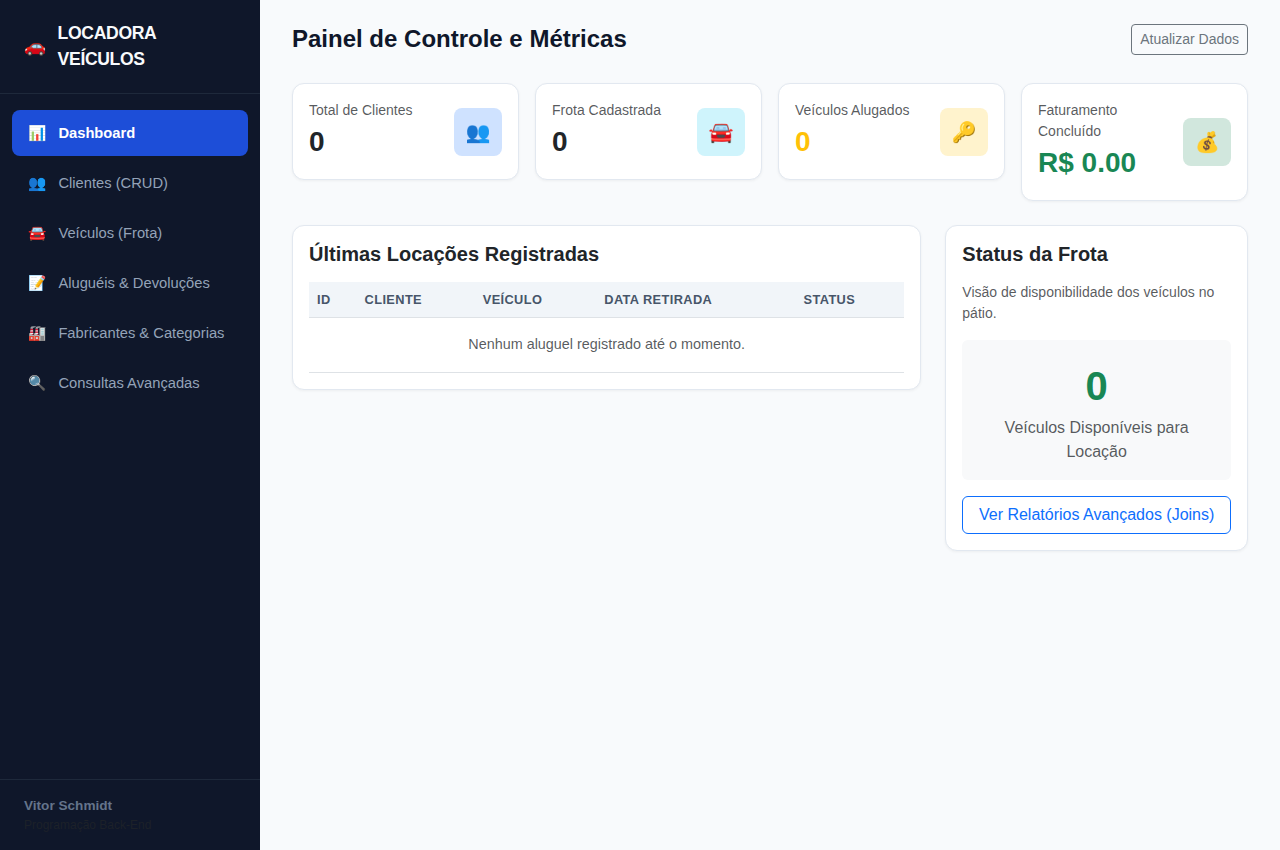
\includegraphics[width=0.92\textwidth]{figuras/01_dashboard.png}
\caption{Wireframe do Dashboard Executivo com indicadores e contratos recentes.}
\label{fig:wireframe_dashboard}
\end{figure}

Para a etapa analítica do sistema, projetou-se um wireframe específico baseado em abas tabulares (\textit{Tabs}), permitindo que o gestor alterne com facilidade entre os cinco relatórios relacionais avançados sem poluição visual, conforme ilustrado na Figura~\ref{fig:wireframe_consultas}.

\begin{figure}[H]
\centering
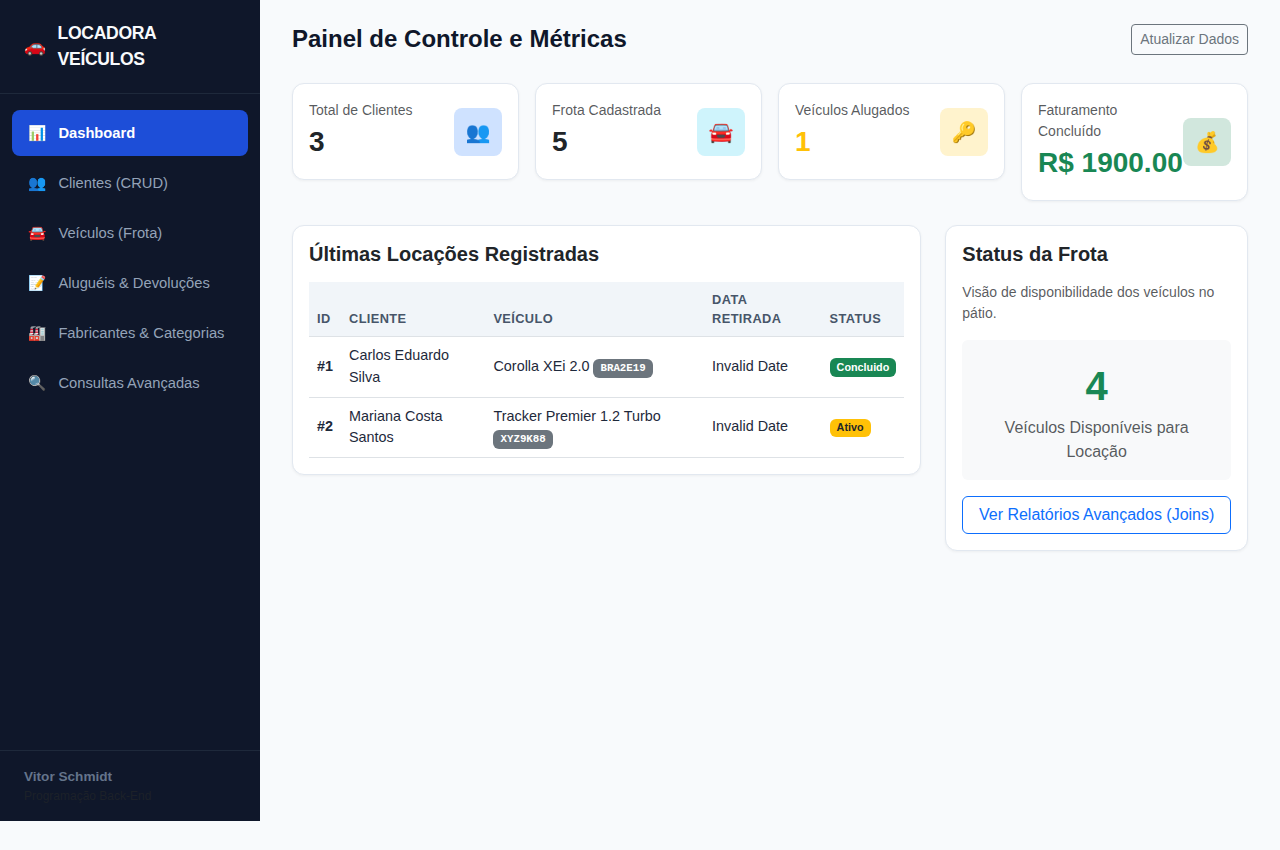
\includegraphics[width=0.92\textwidth]{figuras/06_consultas_avancadas.png}
\caption{Wireframe do módulo de Consultas Avançadas e Relatórios em abas.}
\label{fig:wireframe_consultas}
\end{figure}

O projeto completo de wireframes encontra-se compartilhado publicamente no Figma através do link oficial:\\
\url{https://www.figma.com/design/4RvUybZX26RIYfpTQJoJzv/Trabalho-Pr%C3%A1tico-2?node-id=0-1&t=VaKG7JrY3j0xc9lp-1}

\section{Implementação da Camada Front-End}

A camada cliente foi desenvolvida sob o paradigma de Single-Page Application (SPA) pura, concentrada no diretório \texttt{frontend/}. Optou-se deliberadamente pelo não uso de frameworks JavaScript pesados (como Angular ou React), assegurando leveza, carregamento imediato e portabilidade nativa em qualquer navegador web moderno.

\subsection{Pilha Tecnológica e Estrutura de Arquivos}
A estrutura do front-end foi dividida em três pilares:
\begin{itemize}
    \item \textbf{Estruturação e Estilo:} O arquivo \texttt{index.html} utiliza HTML5 semântico com seções alternáveis (\texttt{view-dashboard}, \texttt{view-clientes}, etc.). O framework Bootstrap 5.3 gerencia o grid responsivo e os componentes visuais, enquanto \texttt{css/style.css} personaliza cartões, tipografia, badges e sombras.
    \item \textbf{Serviço de Comunicação REST (\texttt{js/api.js}):} Classe estática \texttt{ApiService} encapsulando chamadas assíncronas via \texttt{fetch()}. Gerencia serialização JSON, envio de cabeçalhos padronizados e interceptação de erros HTTP, traduzindo falhas de rede em notificações amigáveis.
    \item \textbf{Controlador de Aplicação (\texttt{js/app.js}):} Mantém o estado global em memória (\texttt{AppState}), gerencia eventos de navegação, disparo de modais, escutas de filtros e operações de CRUD.
    \item \textbf{Módulo de Consultas Analíticas (\texttt{js/consultas.js}):} Responsável por parametrizar e despachar as chamadas às cinco consultas avançadas com junções relacionais.
\end{itemize}

\subsection{Validações em Tempo Real e Prevenção de Duplo Envio}
Para garantir a integridade dos dados antes do tráfego de rede, foram incorporadas máscaras dinâmicas de digitação nos campos críticos:
\begin{itemize}
    \item \textbf{CPF do Cliente:} Máscara automática formatando o padrão \texttt{000.000.000-00} com limite rígido de 14 caracteres (11 dígitos numéricos), aplicada tanto no modal de cadastro quanto no campo de filtro.
    \item \textbf{Telefone:} Formatação em tempo real no padrão \texttt{(00) 00000-0000} (15 caracteres para celulares) ou \texttt{(00) 0000-0000} (14 caracteres para fixos).
    \item \textbf{CNH:} Validação numérica estrita com limite máximo de 11 caracteres.
\end{itemize}

Adicionalmente, todos os formulários receberam mecanismo de proteção contra múltiplos envios (duplo clique): ao submeter um formulário, o botão de confirmação é desabilitado instantaneamente e recebe um indicador giratório (\textit{spinner}) com o texto ``Salvando...'', sendo reabilitado somente após a conclusão da requisição na cláusula \texttt{finally}.

\section{Resultados e Integração das Consultas com Joins}

A aplicação foi integrada com êxito à API em execução local. A Figura~\ref{fig:real_dashboard} ilustra a tela de Dashboard do front-end em produção, exibindo dados computados diretamente do banco relacional, incluindo totalizador de frota, contagem de locações ativas e faturamento acumulado.

\begin{figure}[H]
\centering
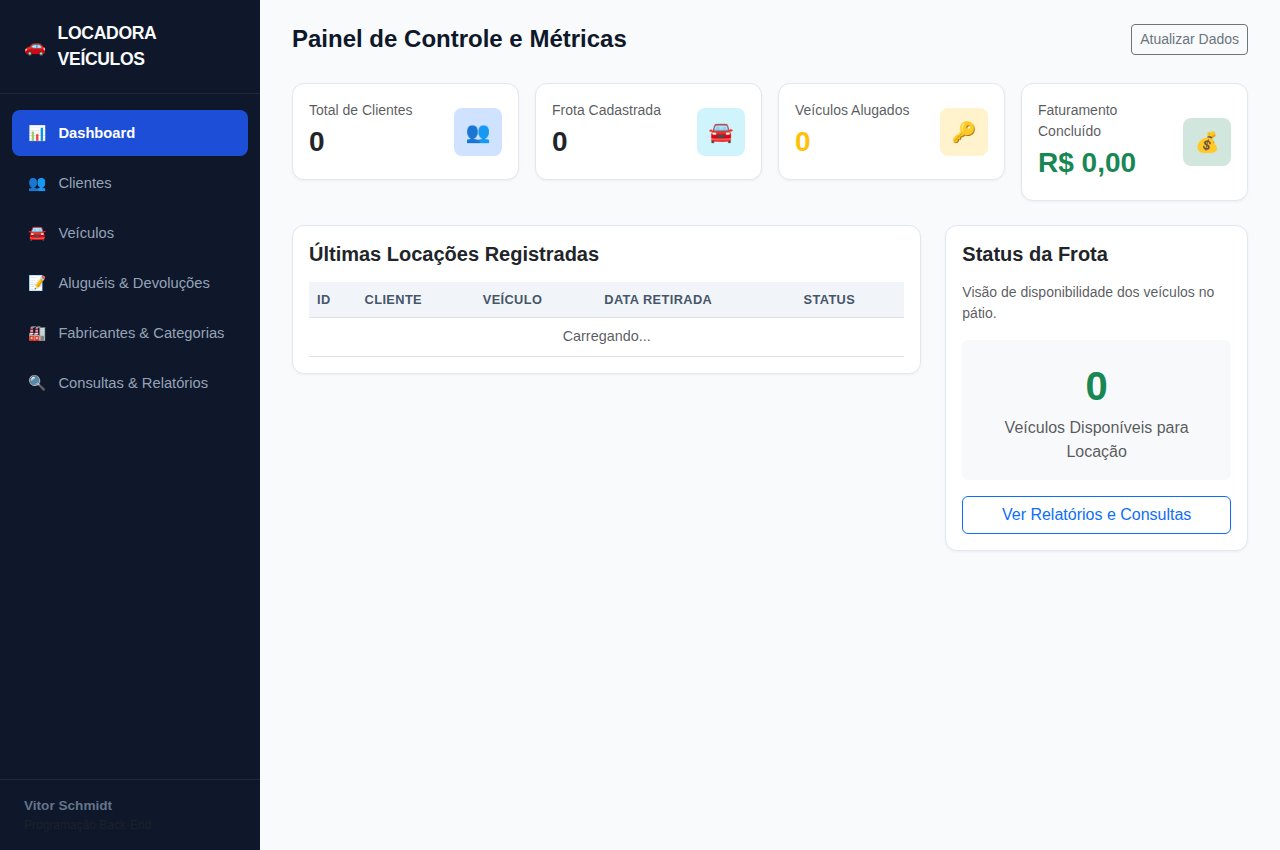
\includegraphics[width=0.92\textwidth]{figuras/frontend_dashboard.png}
\caption{Dashboard da aplicação integrada em tempo real via API RESTful.}
\label{fig:real_dashboard}
\end{figure}

Na gestão operacional de clientes, a Figura~\ref{fig:real_clientes} evidencia a interface com suporte a busca simultânea em múltiplos campos (Nome e CPF com máscara), permitindo a localização ágil de locatários e a execução de operações completas de alteração e exclusão.

\begin{figure}[H]
\centering
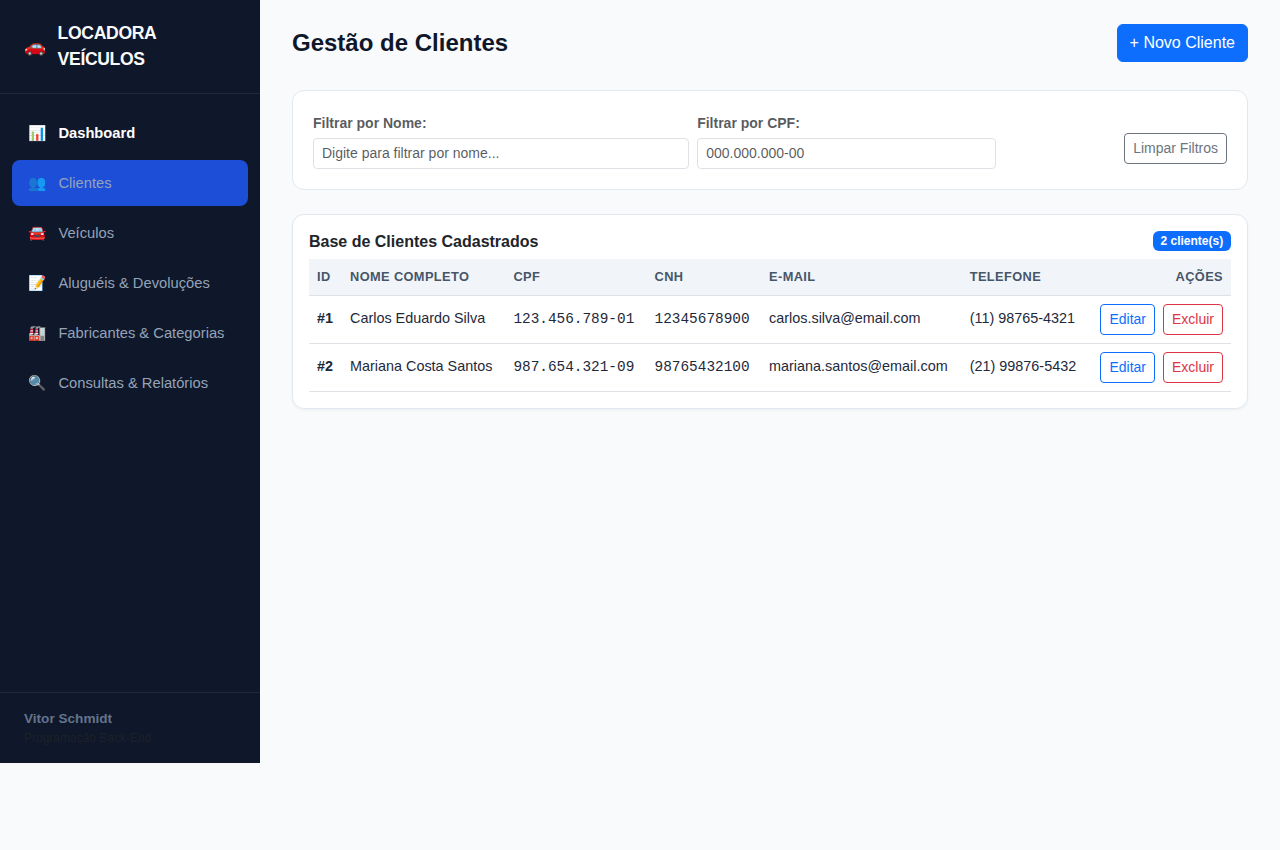
\includegraphics[width=0.92\textwidth]{figuras/frontend_clientes.png}
\caption{Interface de Gestão de Clientes com filtro duplo e máscaras ativas.}
\label{fig:real_clientes}
\end{figure}

\subsection{Demonstração e Mapeamento das Consultas com Joins}

Para cumprir a exigência mandatória de pelo menos cinco consultas utilizando junções relacionais (\textit{INNER JOIN} e \textit{LEFT JOIN}), desenvolveu-se o painel de Consultas Avançadas. A Tabela~\ref{tab:consultas} detalha a correlação técnica de cada consulta implementada.

\begin{table}[H]
\centering
\caption{Mapeamento das 5 consultas relacionais avançadas integradas ao front-end.}
\label{tab:consultas}
\vspace{2mm}
\footnotesize
\begin{tabular}{lp{4.2cm}lp{3.5cm}}
\toprule
\textbf{Consulta} & \textbf{Rota da API (Endpoint)} & \textbf{Tipo de Junção} & \textbf{Objetivo no Negócio} \\
\midrule
\textbf{Filtro 1} & \texttt{/api/Veiculos/disponiveis} & \textit{INNER JOIN} & Veículos livres filtrados por Categoria e Montadora. \\
\textbf{Filtro 2} & \texttt{/api/Alugueis/cliente/\{id\}} & \textit{INNER JOIN} & Histórico consolidado de locações de um cliente. \\
\textbf{Filtro 3} & \texttt{/api/Clientes/relatorio-locacoes} & \textit{LEFT JOIN} & Relação de todos os clientes e faturamento gerado. \\
\textbf{Filtro 4} & \texttt{/api/Veiculos/relatorio-frota} & \textit{LEFT + INNER} & Taxa de ocupação e quilometragem rodada da frota. \\
\textbf{Filtro 5} & \texttt{/api/Alugueis/status-pagamento} & \textit{LEFT + INNER} & Auditoria financeira de contratos quitados e pendentes. \\
\bottomrule
\end{tabular}
\end{table}

A Figura~\ref{fig:real_consultas} exibe a tela de Consultas Avançadas em operação, demonstrando a renderização limpa e profissional dos dados retornados pelas junções SQL, sem exposição desnecessária de termos técnicos ao usuário final.

\begin{figure}[H]
\centering
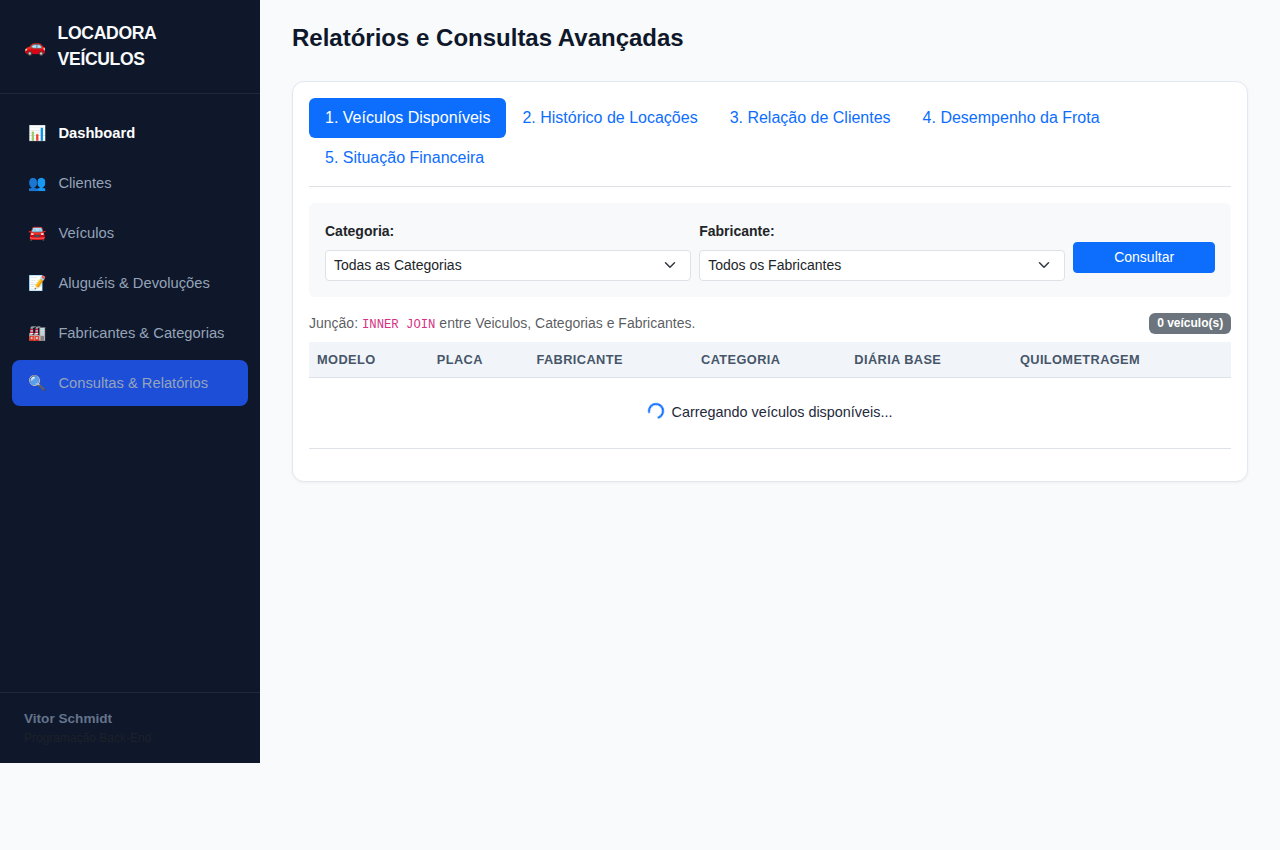
\includegraphics[width=0.92\textwidth]{figuras/frontend_consultas.png}
\caption{Painel de Consultas Avançadas exibindo resultados das junções relacionais.}
\label{fig:real_consultas}
\end{figure}

\section{Considerações Finais}

O Trabalho Prático 2 alcançou plenamente os objetivos pedagógicos e técnicos propostos pela disciplina de Programação Back-End. A construção do front-end a partir de wireframes no Figma proporcionou uma transição consistente entre a fase de design de interação e a codificação de software.

A arquitetura em SPA aliada à Fetch API permitiu uma interface responsiva, com validações cadastrais instantâneas e tratamento elegante de erros de banco de dados. A integração ponta a ponta com a API em C# (.NET 8) comprovou a eficácia do desacoplamento arquitetural, mantendo a integridade referencial por meio de consultas otimizadas com \textit{INNER JOIN} e \textit{LEFT JOIN}.

\section*{Repositório e Wireframes}
\begin{itemize}
    \item \textbf{Repositório no GitHub:} \url{https://github.com/vitor-schmidt-ribeiro/locadora-veiculos}
    \item \textbf{Wireframes no Figma:} \url{https://www.figma.com/design/4RvUybZX26RIYfpTQJoJzv/Trabalho-Pr%C3%A1tico-2?node-id=0-1&t=VaKG7JrY3j0xc9lp-1}
\end{itemize}

\begin{thebibliography}{6}

\bibitem{elmasri2011}
Elmasri, R. e Navathe, S.~B. (2011).
\newblock {\em Sistemas de Banco de Dados}.
\newblock Pearson Addison Wesley, São Paulo, 6ª edição.

\bibitem{pressman2016}
Pressman, R.~S. e Maxim, B.~R. (2016).
\newblock {\em Engenharia de Software: Uma Abordagem Profissional}.
\newblock McGraw-Hill, Porto Alegre, 8ª edição.

\bibitem{sommerville2011}
Sommerville, I. (2011).
\newblock {\em Engenharia de Software}.
\newblock Pearson, São Paulo, 9ª edição.

\bibitem{microsoftdotnet}
Microsoft (2024).
\newblock {\em Documentação Oficial do ASP.NET Core e Entity Framework Core}.
\newblock Microsoft Learn. Disponível em: \url{https://learn.microsoft.com/aspnet/core}.

\bibitem{bootstrap5}
Bootstrap Team (2024).
\newblock {\em Bootstrap 5 Documentation: Responsive Front-End Framework}.
\newblock Disponível em: \url{https://getbootstrap.com/docs/5.3/}.

\bibitem{sbc2024}
Sociedade Brasileira de Computação (SBC) (2024).
\newblock {\em Padrões para Publicação de Artigos em Conferências da SBC}.
\newblock Disponível em: \url{https://www.sbc.org.br}.

\end{thebibliography}

\end{document}
